\documentclass[journal, a4paper]{IEEEtran}

% Import packages
\usepackage{graphicx}
\usepackage{url}
\usepackage{amsmath}
\usepackage[svgnames]{xcolor}
\usepackage{listings}

\lstset{language=R,
    basicstyle=\small\ttfamily,
    stringstyle=\color{DarkGreen},
    otherkeywords={0,1,2,3,4,5,6,7,8,9},
    morekeywords={TRUE,FALSE},
    deletekeywords={data,frame,length,as,character},
    keywordstyle=\color{blue},
    commentstyle=\color{DarkGreen},
}

\begin{document}
	\title{Bayesian Stats Techniques and Models Capstone:\\ Weight Loss Analysis}
	\author{Simon Thornewill von Essen\\ Dates: 07/02/2020 - 11/02/2020
	\thanks{}}
	\markboth{}{}
	\maketitle


\begin{abstract}

The difficulty with weight loss can sometimes be understanding if the change in weight over time is real and not due to random chance. In this report, bayesian
ANOVA is used to determine whether there is significant weight loss between two months measured using a smart scale. It was found that the means between the two
months were very different, producing posterior distributions for the means of the two months that barely overlapped. As such, it has been concluded that 
significant weight loss was achieved.

\end{abstract}

\section{Introduction}
\IEEEPARstart{L}{ately,} I have been trying to lose weight. One question that I have is whether I have had any significant weight loss over the past two months.
In order to evaluate this problem, I have decided to weigh myself using a RENPHO smart scale over the course of Janurary and Feburary 2020. This scale not only
measures my weight, but also tracks other metrics such as body fat percentage, bone density, blood protein percentage and so on.\\ 

What I did was weigh myself every day, once in the morning and once in the evening. Although your weight tends to be most consistent in the morning and you
tend to gain ``weight'' by the evening, I weighed myself twice to get a better picture of what my average weight for the day was.\\

Luckily, since this data is generated by my self, there are no issues with the data such as missing values. The only issue was removing units such as "kg" from
the values and renaming the columns so that they work better within a coding environment. As such, there were not a lot of challenges with aquiring the data
itself. Perhaps the only issue was cleaning it withing python instead of using R, because my python skills are far sharper than my R skills.\\
	
\section{Data Exploration}

Before doing any modeling I wanted to do some quick plots to get a sense of the data that I was interested in. I was mostly interested in how my weight changed
over time, which means that I was primarily concerned with this this metric instead of all of the columns that I was able to make for the dataset. In 
retrospect, it might have been a good idea to drop some of the columns that were estimated by the RENPHO smart scanner. (We'll see why I think that in the next
subsection.)\\

Note that these plots can be found in the appendix section so that they do not break the flow of the text.

\subsection{Body Fat Percentage vs. Body Weight}

One of the things I was most interested in was the change in body fat percentage as a function of Body Weight. We can see in this plot that the relationship 
between body weight and body fat percentage if roughly linear. This is something that we do not expect because  as a person's body weight decreases, the amount 
of weight they need to drop to reduce their fat further is smaller and \textit{vice. versa.}

\subsection{Month over Month Change in Body Weight}

Looking at the month over month (MoM) change in body weight, we can see that in Janurary there is a large variability in body weights whereas the second month
is more consistent, with mean values being weound 81 kg for Janurary and roughly 80 kg in Feburary. It seems like there was meaningful weight loss, given that 
the boxes themselves do not overlap, but if you include the tails then there is still some overlap.

\subsection{Week over Week Change in Body Weight}

For the week over week (WoW) change in body weight we can see the story unfold a little more clearly. We can see that in the 2nd week of 2020 that the 
variability is quite high, but the weight stabilises a little more from the 3rd week onwards. The difference between weeks 4 and 5 are quite profound, with week
6 increasing again in variability.\\

It should be noted that during the week with the most weight loss I was using itermittent fasting instead of simple caloric restriction. While I found that it 
was good at the start, I found that my weight loss plateaued quickly. I think this was because I was losing weight too quickly, causing my body to go into what
is known as ``starvation mode'' to try and retain the body fat that I was losing.

\section{Modeling}

\subsection{Model Postulation}

In order to find out whether the weight loss was meaningful between the two months, I want to do an ANOVA test to see if this was really the case. ANOVAs test
for proportions between the intra-group and inter-group variances to see if a categorisation is ``meaningful''. This test is appropriate because it tests for
data that have categorical and continuous variables, which is exactly what we have.\\

ANOVA models assume that data is normally distributed and that each group (in this case, we have two) and that each group has its own mean. Note that it is also
possible for each group to have its own variance as well. To start, we will assume that each group has its own variance but we can already see from our 
exploratory data analysis that this assumption may not actually hold in this case. We are interested in seeing the differences between the posterior
distributions of the means.\\

Thus, using the description above we can write the model likelihood where we assume the variances between groups are the same:\\

$$y_i | g_i,  \tilde\mu, \sigma^2 \overset{\text{iid}}{\sim} N(\mu_g, \sigma^2)$$

Where the prior distributions for the means and variances are as follows:

$$\mu_j \overset{\text{iid}}{\sim} N\left(0.0, \frac{1.0}{10^6}\right)$$
$$\sigma^2 \overset{\text{iid}}{\sim} \frac{1}{\textrm{Gamma}(\frac{1.0}{2.0}, \frac{1.0 \times 1.0}{2.0})} $$\\

For the prior distributions, I chose uninformative priors. Where the uninformative prior for the mean of a normal distribution is also normally distributed with
a mean of zero and a very large variance. \textit{Note: JAGS uses a precision parameter instead of variance, which is why the reciprocal was taken.}\\

Furthermore, the prior distribution for the $\sigma^2$ parameter is drawn from an inverse gamma distribution, with a prior sample size of 1 and a prior guess of
1 as well. Note that this is also meant to be uninformative.

\subsection{Model Fitting}

Now that the model has been defined, it needs to be fit in R with RJAGS. The code for the model string is as follows:\\

\begin{lstlisting}
model{
  for(i in 1:length(y)){
    y[i] ~ dnorm(mu[month[i]], prec)
  }
  
  for(j in 1:max(month)){
    mu[j] ~ dnorm(0.0, 1/1.0e6)
  }
  
  prec ~ dgamma(1.0/2.0, 1.0*1.0/2.0)
  sig = sqrt(1.0 / prec)
}
\end{lstlisting}

Where y is equal to my measured weight in kilograms, and month is the month when the measurement was taken. The model was instantiated with three chains and 
updated for 1,000 iterations before sampling from each of the chains 1000 times.

\subsection{Convergence Diagnostics}

Before analysing the posterior sample to answer the question we set out with, it's a good idea to see whether the chain converged. This will be assessed using
a number of diagnostic tools.\\

\begin{itemize}
	\item Trace plots of the samples drawn from the posterior distribution.
	\item Gelman-Rubin diagnostics.
	\item Autocorrelation diagnostics. (Including visualisation.)
	\item Effective sample sizes of each parameter.
\end{itemize}

\ \\

The trace plots for the analysis can be found in the appendix under fig. \ref{fig:4}. As mentioned in the caption, the chains seem to be sampling from the 
posterior distribution well, without spending a lot of time in one area or wandering around the space.\\

This is confirmed by the Gelman-Rubin diagnostics, which are printed below:\\

\begin{verbatim}
Potential scale reduction factors:

      Point est. Upper C.I.
mu[1]          1          1
mu[2]          1          1
sig            1          1

Multivariate psrf

1
\end{verbatim}

From these diagnostics, we can conclude that there is no need to do any thinning of the chains, which is further evidence that the chains are sampling well from
the posterior distribution.\\

Next, let's have a look at the autocorrelation diagnostics:\\

\begin{verbatim}
               mu[1]        mu[2]        sig
Lag 0   1.0000000000  1.000000000 1.00000000
Lag 1  -0.0006874275  0.005679199 0.06212891
Lag 5  -0.0001819209 -0.012440970 0.02044134
Lag 10 -0.0136230695  0.020004604 0.01804867
Lag 50  0.0207523518  0.030407469 0.00853365
\end{verbatim}

We can see there, as well as what is visalised in the appendix in fig. \ref{fig:5} that there is a lot of autocorrelation for the first iteration, but the chain
quickly reduces its autocorrelation to zero. Once again, this is more evidence that the chain is sampling from the posterior distribution well. There are no
concerns to be made here.\\

Finally, we want to have a look at the effective sample sizes:\\

\begin{verbatim}
   mu[1]    mu[2]      sig 
3000.000 3000.000 2648.149 
\end{verbatim}

We can see here that for the means of the groupings, have a 100\% effective sample size. Note that we have three chains of 1,000 samples, which we combine into
one large sample of 3,000 observations. However, we should note that the standard deviation sample size is roughly 88\%. We already noted that it is unlikely
that the standard deviations between the group distributions are the same based on our visualisations, and this confirms that hypothesis.\\

If we wanted to improve our model, we would consider using separate parameters for the standard deviation for each group. We could confirm that this is really
an improvement by looking at the DIC diagnostics between the models to see which has the lowest penalty. However, this will not be done here because the 
effective sample size seems to be large enough to have some information over our driving question.

\subsection{Tests for Assumptions}

Plots for the residuals can be found in figures \ref{fig:7} and \ref{fig:8}. We can see in both of these plots that the variance between the two groups are 
clearly not the same, which we already knew. To combat this, we will change our model to have two parameters for the standard deviation. The model gets changed
below such that the precision parameter is in side the for loop for each group parameter along with the calculation for the standard deviation:\\

\begin{lstlisting}
model{
  for(i in 1:length(y)){
    y[i] ~ dnorm(mu[month[i]], prec[month[i]])
  }
  
  for(j in 1:max(month)){
    mu[j] ~ dnorm(0.0, 1/1.0e6)
    prec[j] ~ dgamma(1.0/2.0, 1.0*1.0/2.0)
    sig[j] = sqrt(1.0 / prec[j])
  }
}
}
\end{lstlisting}

The trace plot for this model can be found at \ref{fig:6}. We won't run convergence diagnostics because the trace plots look okay and the rest of the 
diagnostics looked good the first time around.\\

Next, we want to analyse which model is better using the DIC value from before. For model one we get the following results:

\begin{verbatim}
Mean deviance:  158.8 
penalty 3.154 
Penalized deviance: 162 
\end{verbatim}

And for the second model we get these results...

\begin{verbatim}
Mean deviance:  152.7 
penalty 4.197 
Penalized deviance: 156.9
\end{verbatim}

We can see that although we have a higher penalty in our second model since it is more complex, the mean deviance is lower because it has explanatory power.
Overall, the penalized deviance for the second model is lower than the first, so we will use this model when doing analysis on the posterior distribution.

\section{Results}

When taking the means $\mu_1$ and $\mu_2$, we can see that $\mu_2$ is smaller 100\% of the time. If you view the posterior distributions for the means in a
visalisation, then you can see that there is no overlap between them. This means that meaningful weightloss has been achieved. We can also see from the 
posterior summary below that the weight in the second month becomes more consistent as well, exactly as we expect.

\begin{verbatim}
          Mean     SD
mu[1]  81.2049 0.1598
mu[2]  79.9153 0.1692
sig[1]  1.0511 0.1120
sig[2]  0.6237 0.1255
\end{verbatim}

However, the real question is if this finding generalises into further weight loss. For this we would want to wait a longer time, perhaps four months or so and
then do another analyis based on those results. Note as well that it would also be good to know what actions caused the weight loss as opposed to analysing 
whether it has taken place in a meaningful way.

\section{Conclusion}

We set out on this analysis to discover if there has been meaningful change of weight as a result of habit changes. It was found that there was a very high 
probability that the differences in means were not due to chance alone, with a mean loss of weight of roughly 1.29 kilograms over the time of measurement. 

\newpage
\onecolumn

\section{Appendix}

\subsection{Figures}

\begin{figure}[h!]
	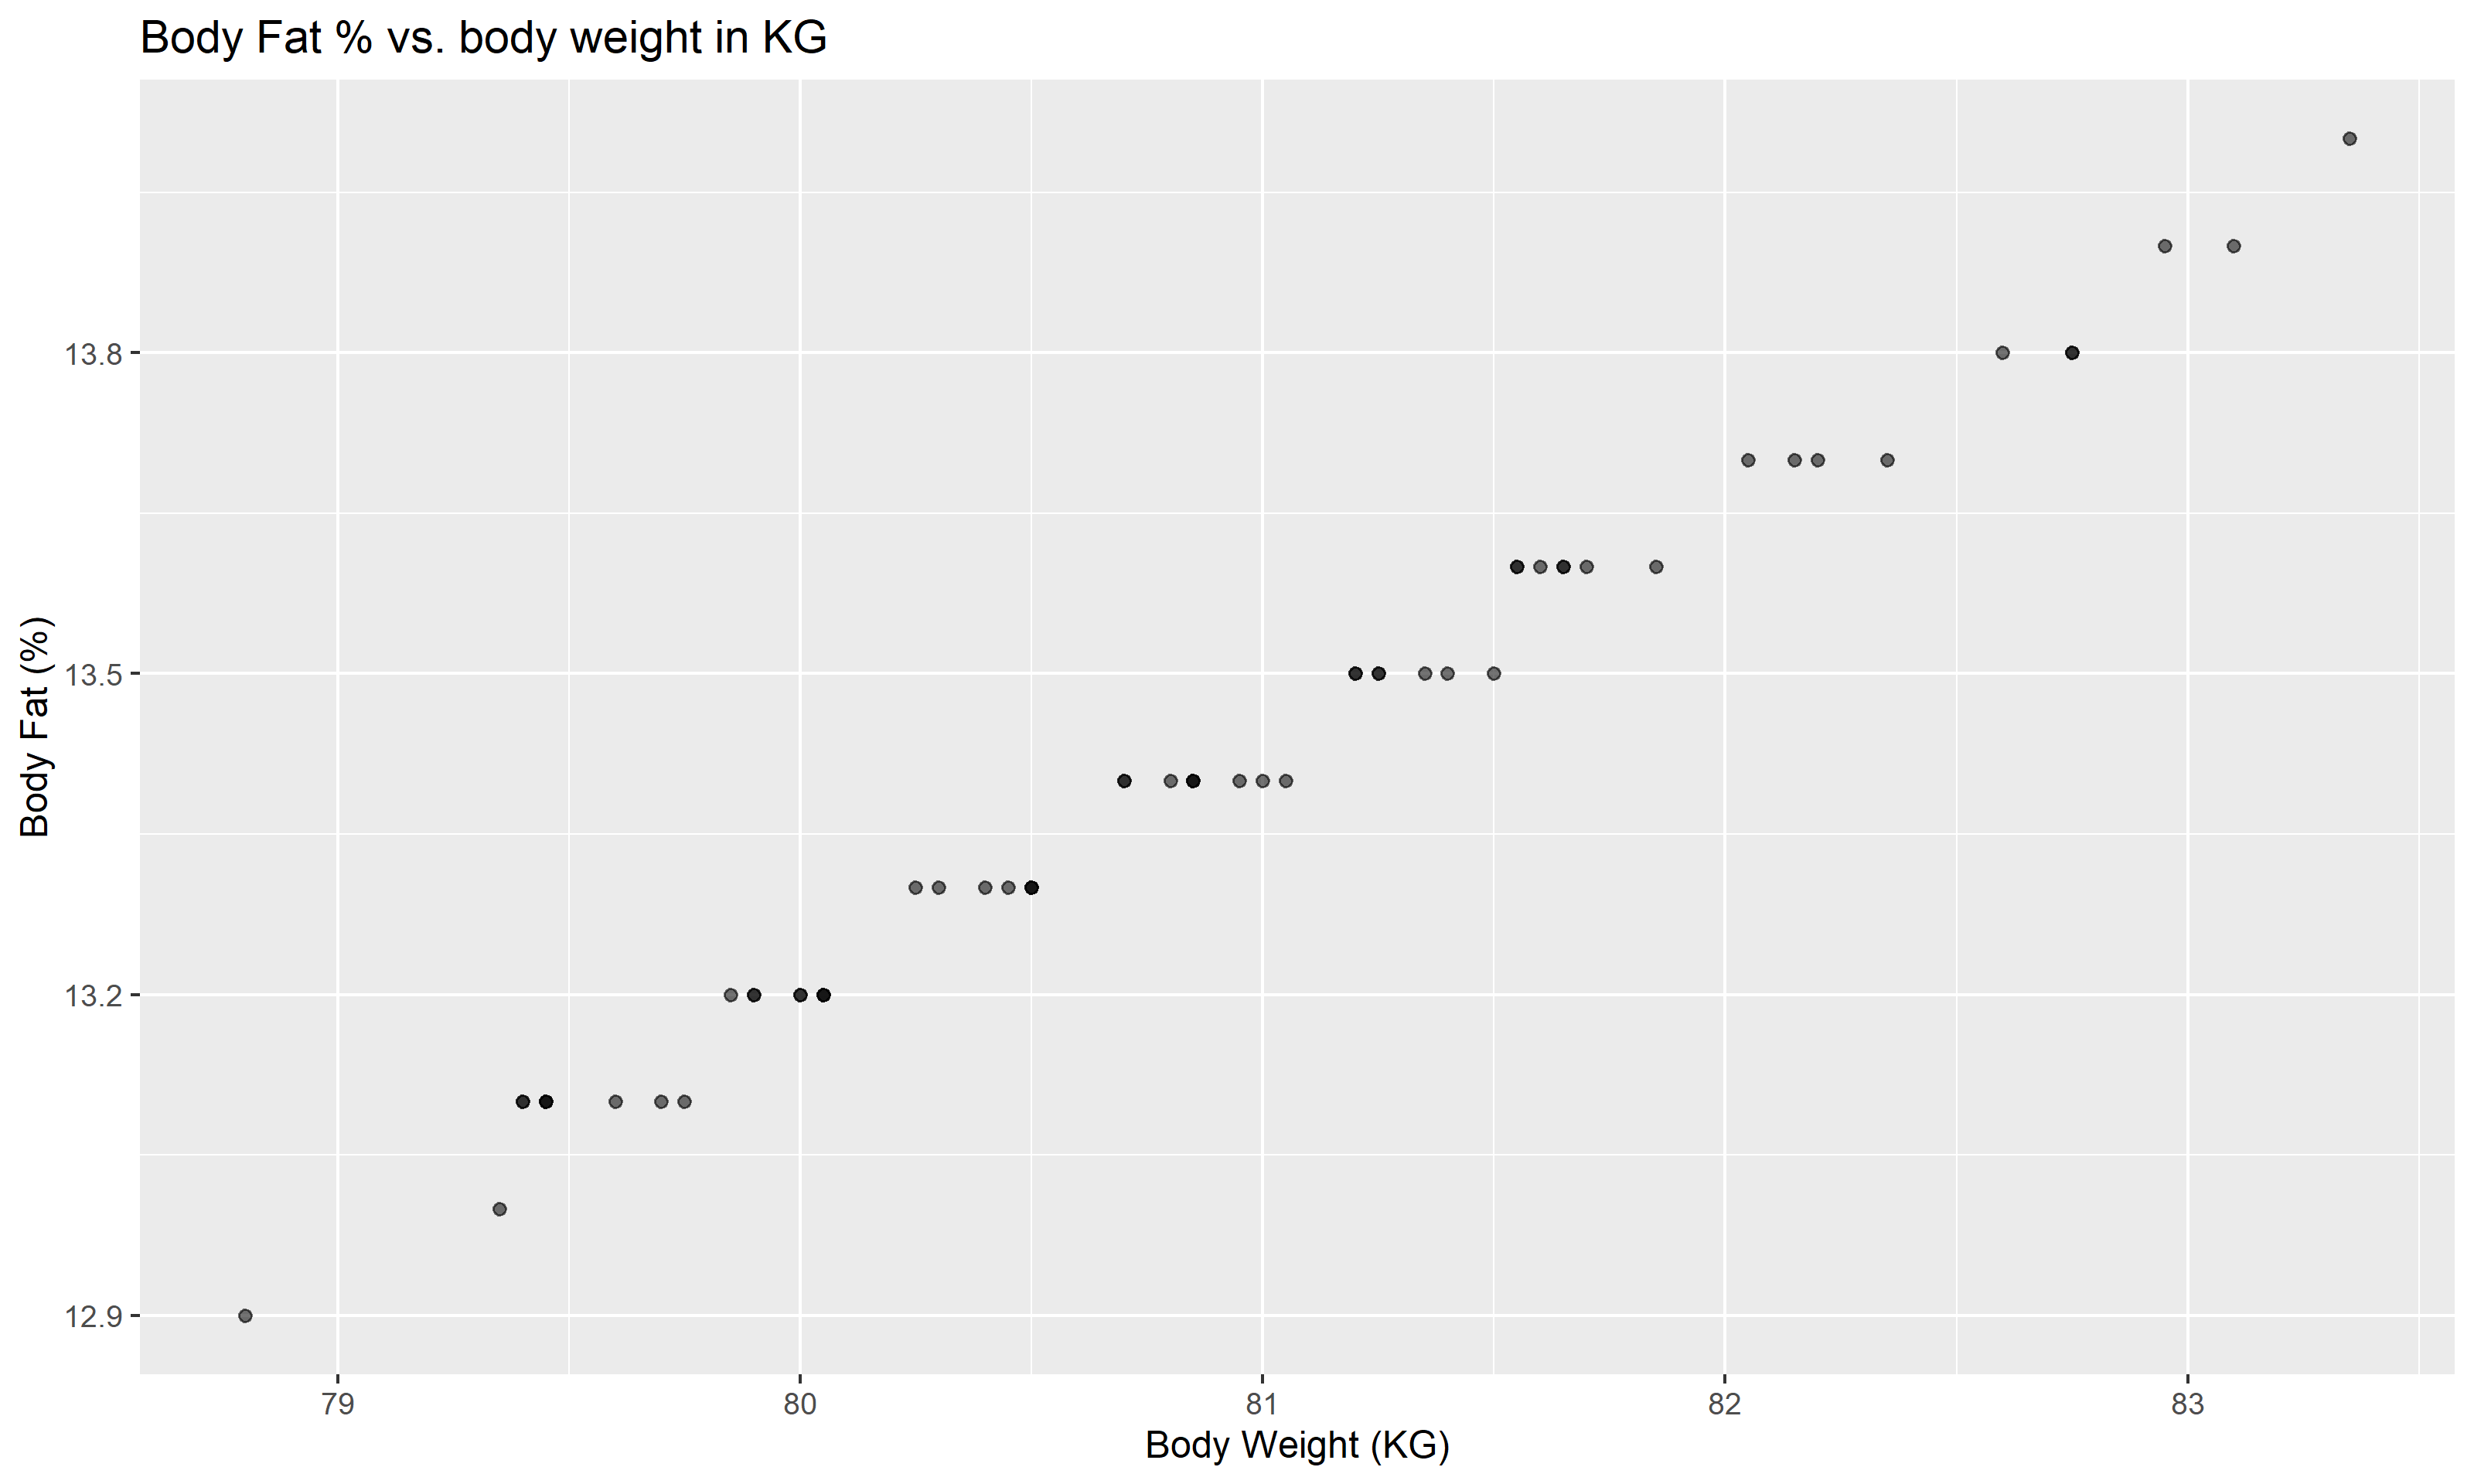
\includegraphics[width=\linewidth]{../plots/01_bf_vs_bw.png}
	\caption{Scatter plot of two numeric values, body fat percentage versus body weight. We can see a linear relationship between the two variables. However,
	it it expected that it only looks linear because of the relatively small body weight range, if I were to measure myself as being extremely under/over weight
	then we would expect the relationship to be non-linear.}
	\label{fig:1}
\end{figure}

\begin{figure}[h!]
	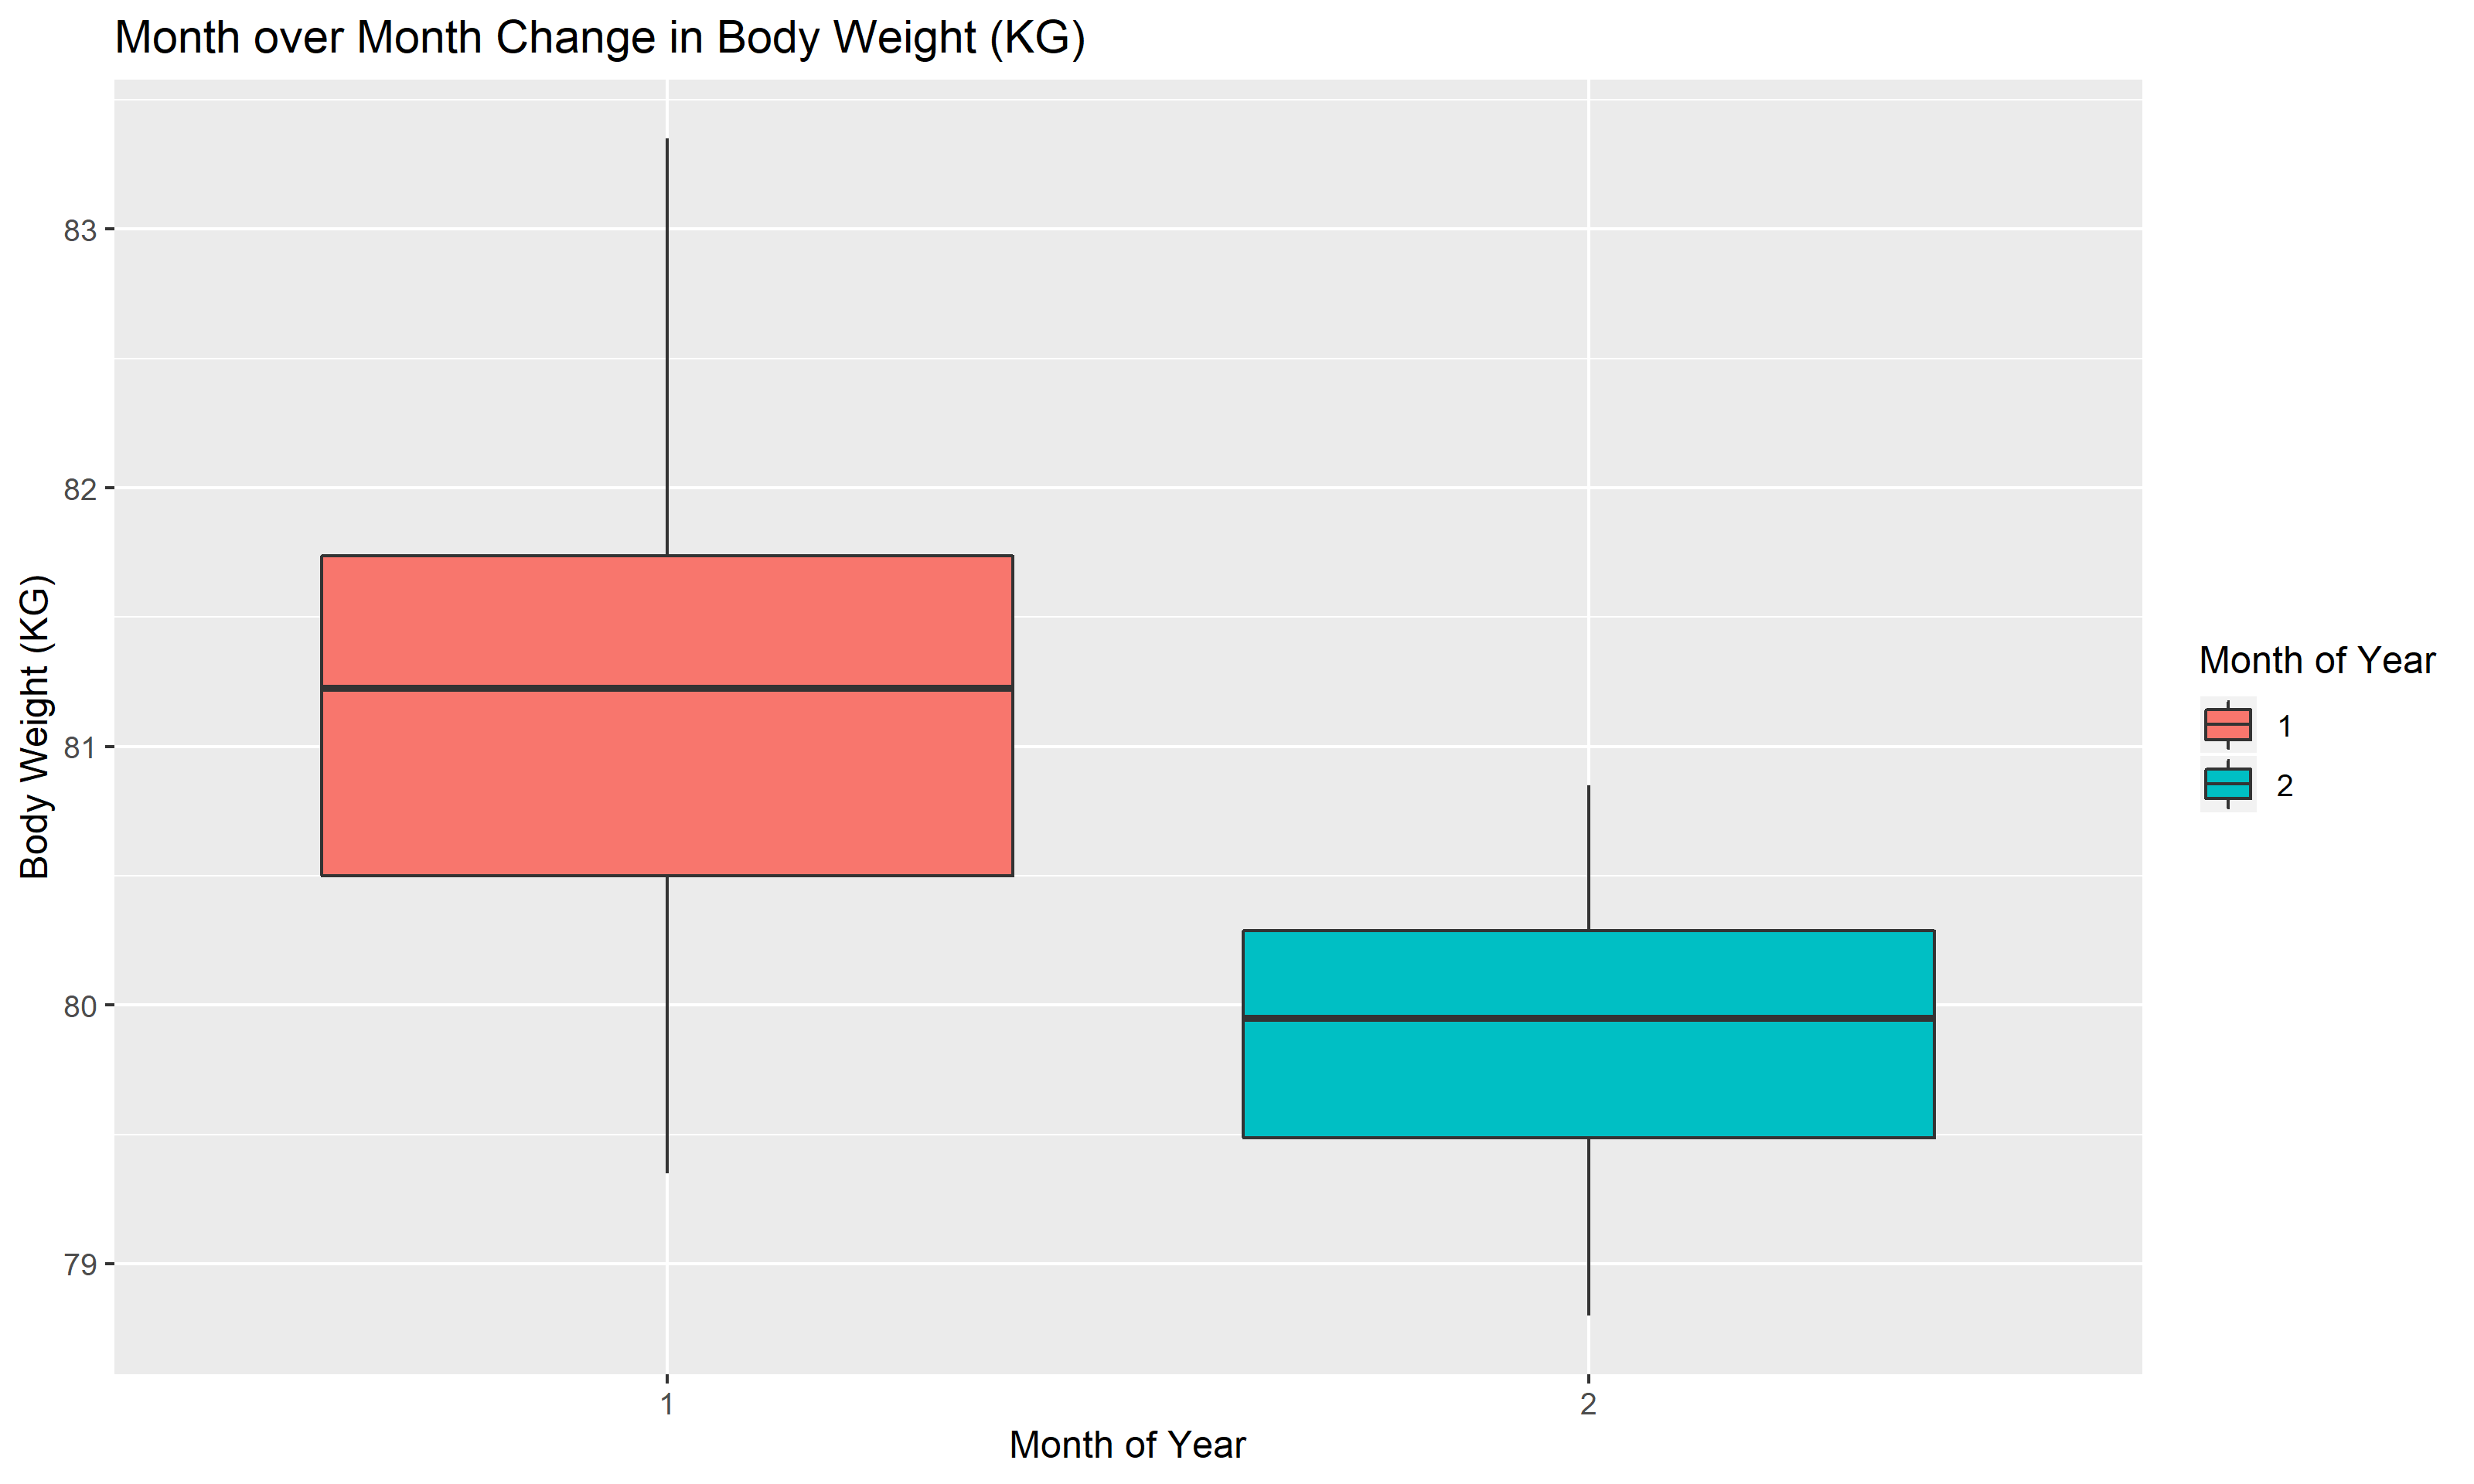
\includegraphics[width=\linewidth]{../plots/02_bw_vs_mnth.png}
	\caption{Boxplot showing change in body weight over the two months where it was measured. We can see that there is certainly a change in body weight, but is
	it meaningfully different?}
	\label{fig:2}
\end{figure}

\begin{figure}[h!]
	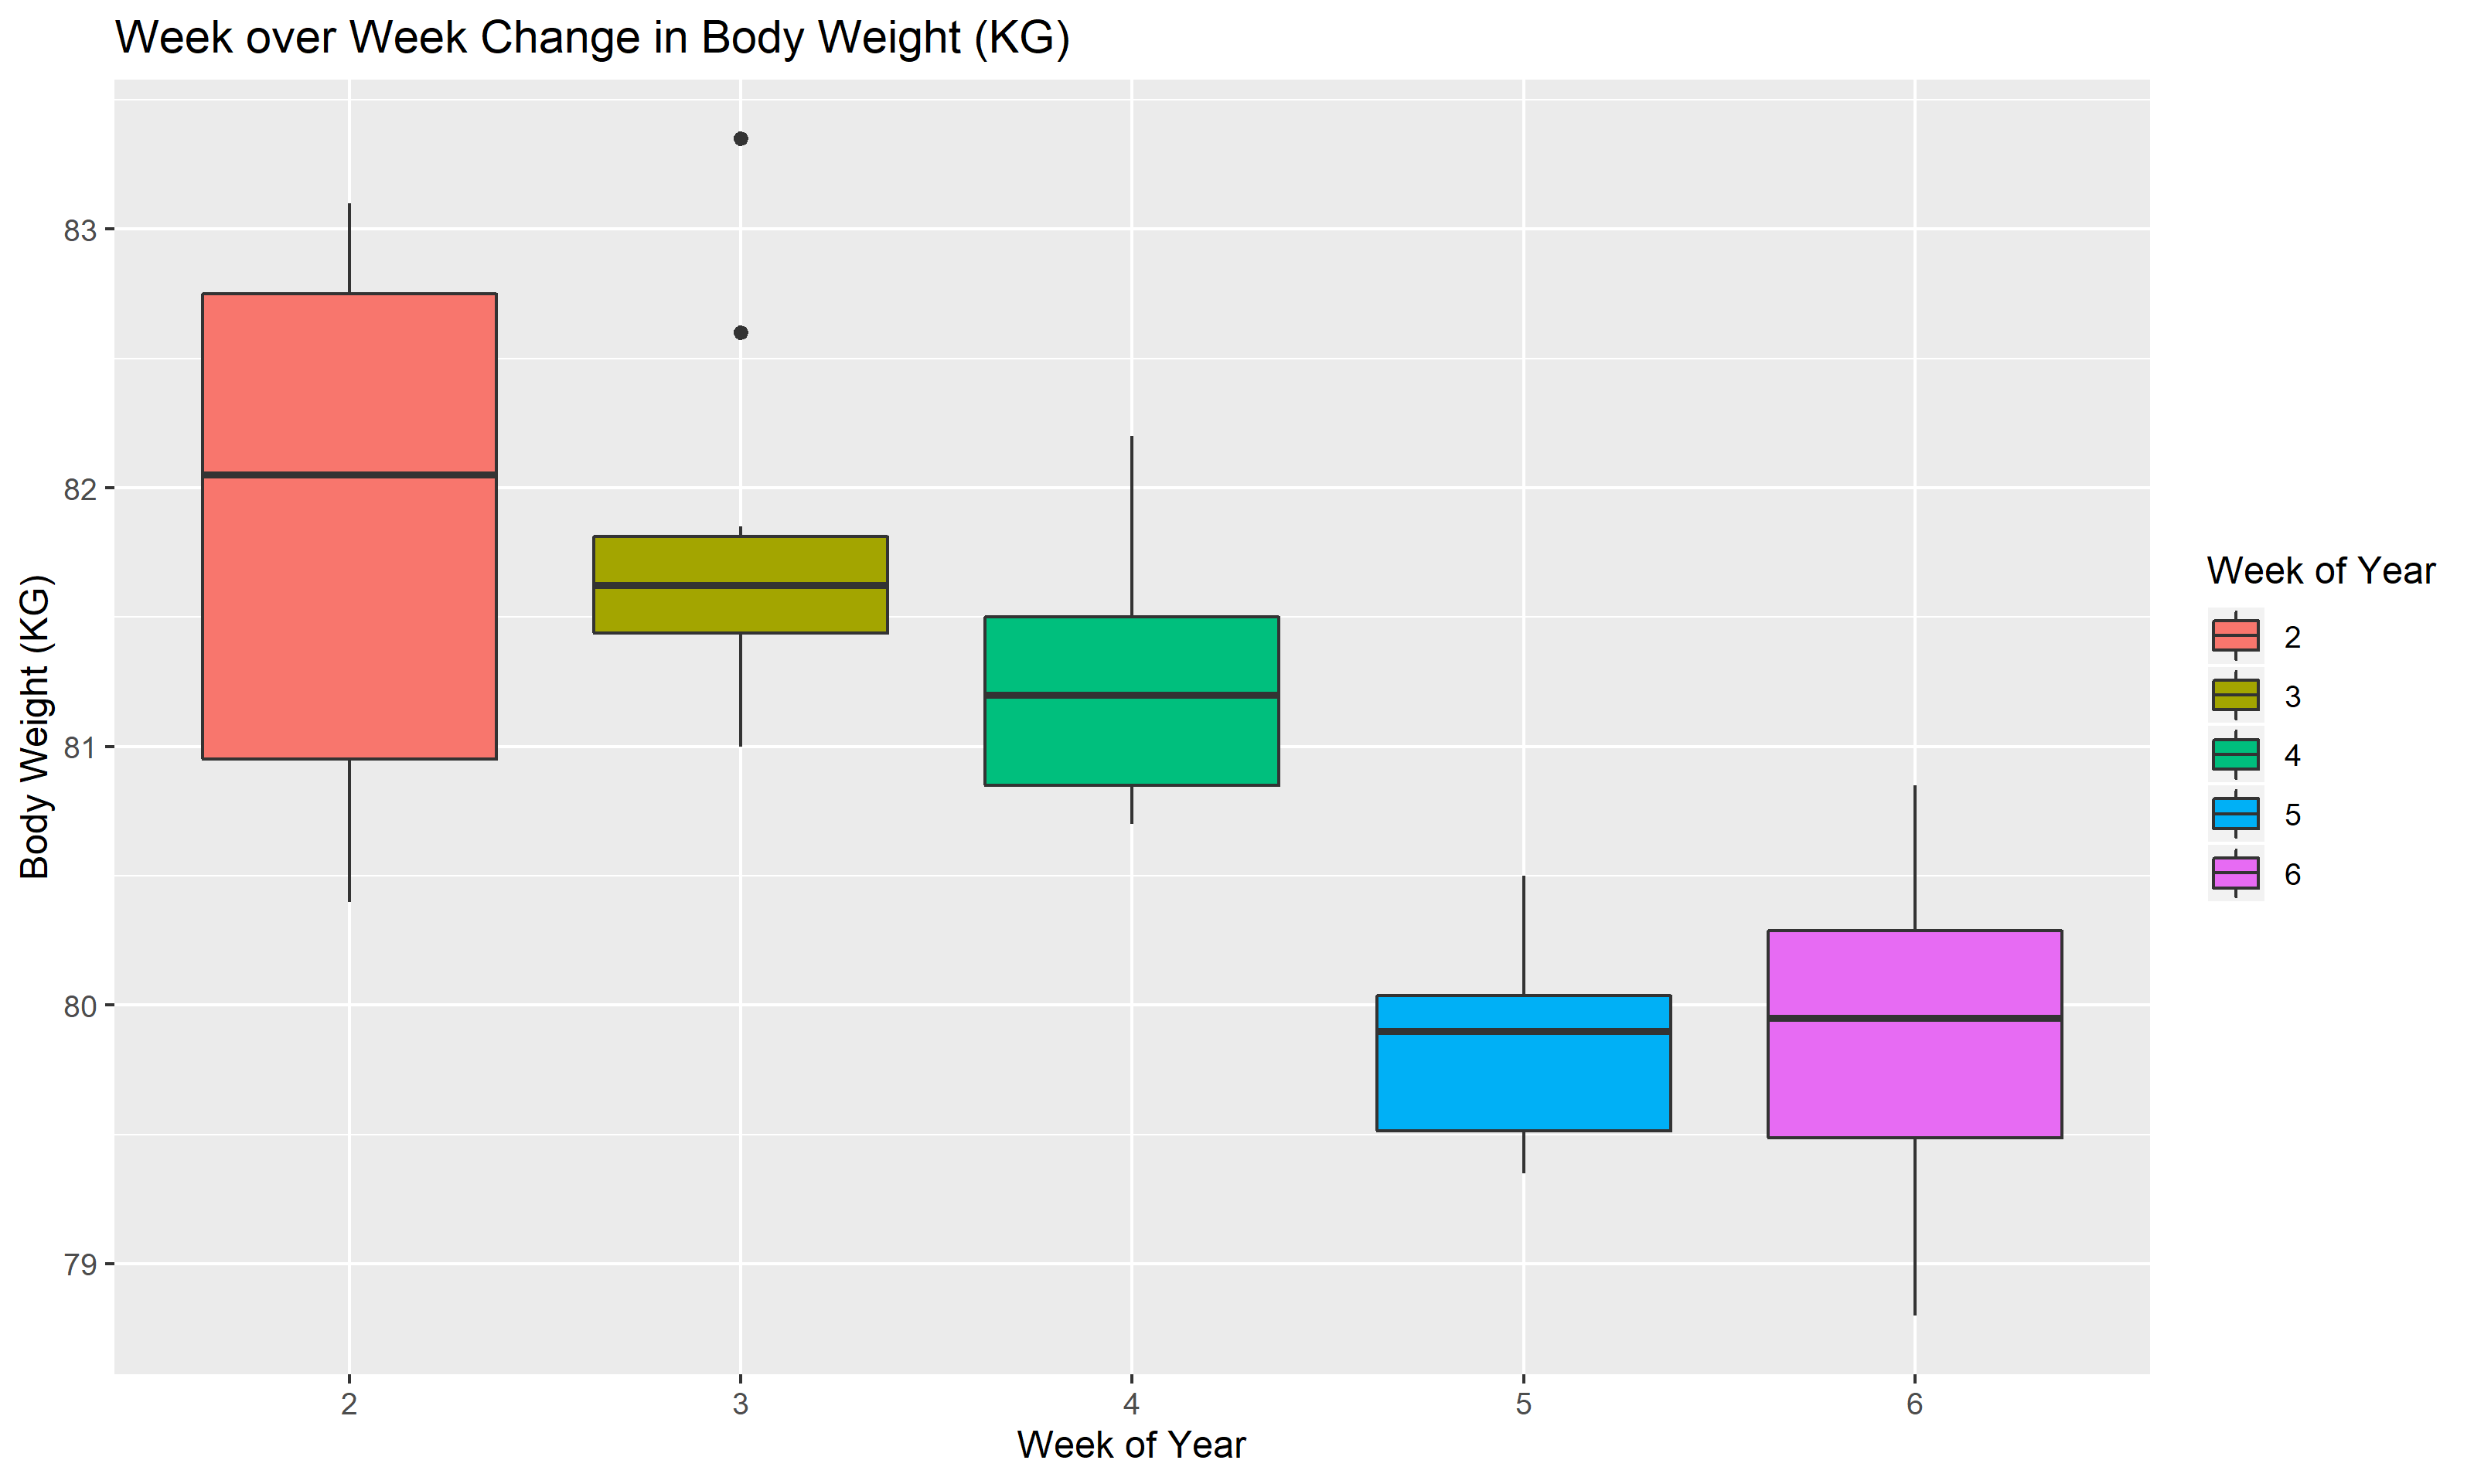
\includegraphics[width=\linewidth]{../plots/03_bw_vs_wk.png}
	\caption{Boxplot showing change in body weight over the weeks where it was measured. In the first week we can see that there were large variations in body
	weight, during weeks 5 and 6 the weight is very different from the start at weights 2 and 3.}
	\label{fig:3}
\end{figure}

\begin{figure}[h!]
	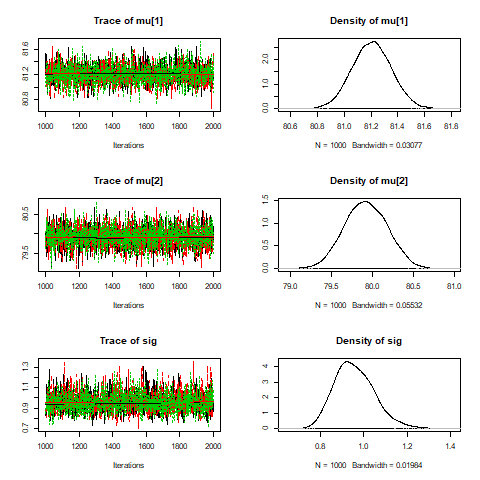
\includegraphics{../plots/04_chains_ANOVA.png}
	\caption{Visualisation of the MCMC chains for the parameters of the ANOVA test. We can see from the trace plots that the sampler is exploring the space
	appropriately, without lingering too long around one area while still converging on one value.}
	\label{fig:4}
\end{figure}

\begin{figure}[h!]
	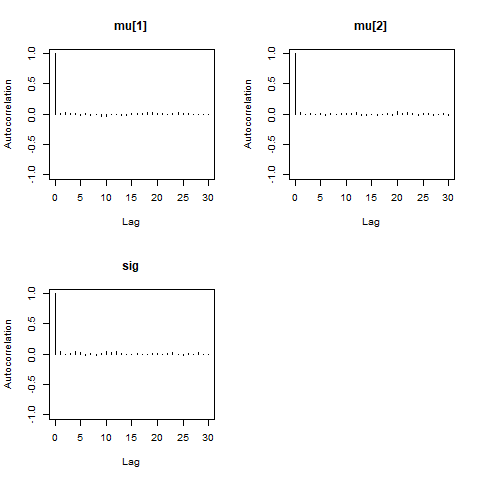
\includegraphics{../plots/05_autocorr.png}
	\caption{Visualisation of the MCMC chain autocorrelations. We can see that there is large autocorrelation at the start but it very quickly dies out. There
	is no cause for concern here.}
	\label{fig:5}
\end{figure}

\begin{figure}[h!]
	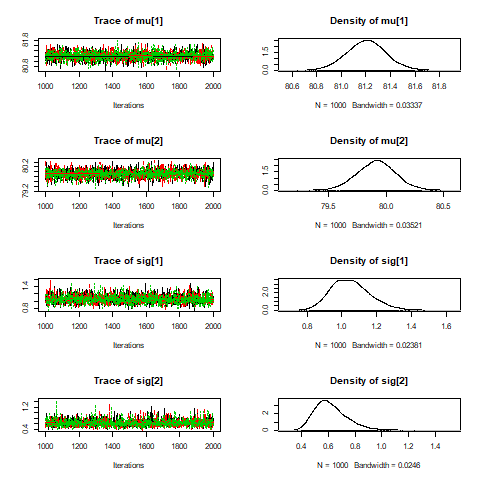
\includegraphics{../plots/04_chains_ANOVA_2.png}
	\caption{Visualisation of the MCMC chains for the parameters of the ANOVA test with separate parameters for standard deviation. We can see from the trace 
	plots that the sampler is exploring the space appropriately, without lingering too long around one area while still converging on one value.}
	\label{fig:6}
\end{figure}

\begin{figure}[h!]
	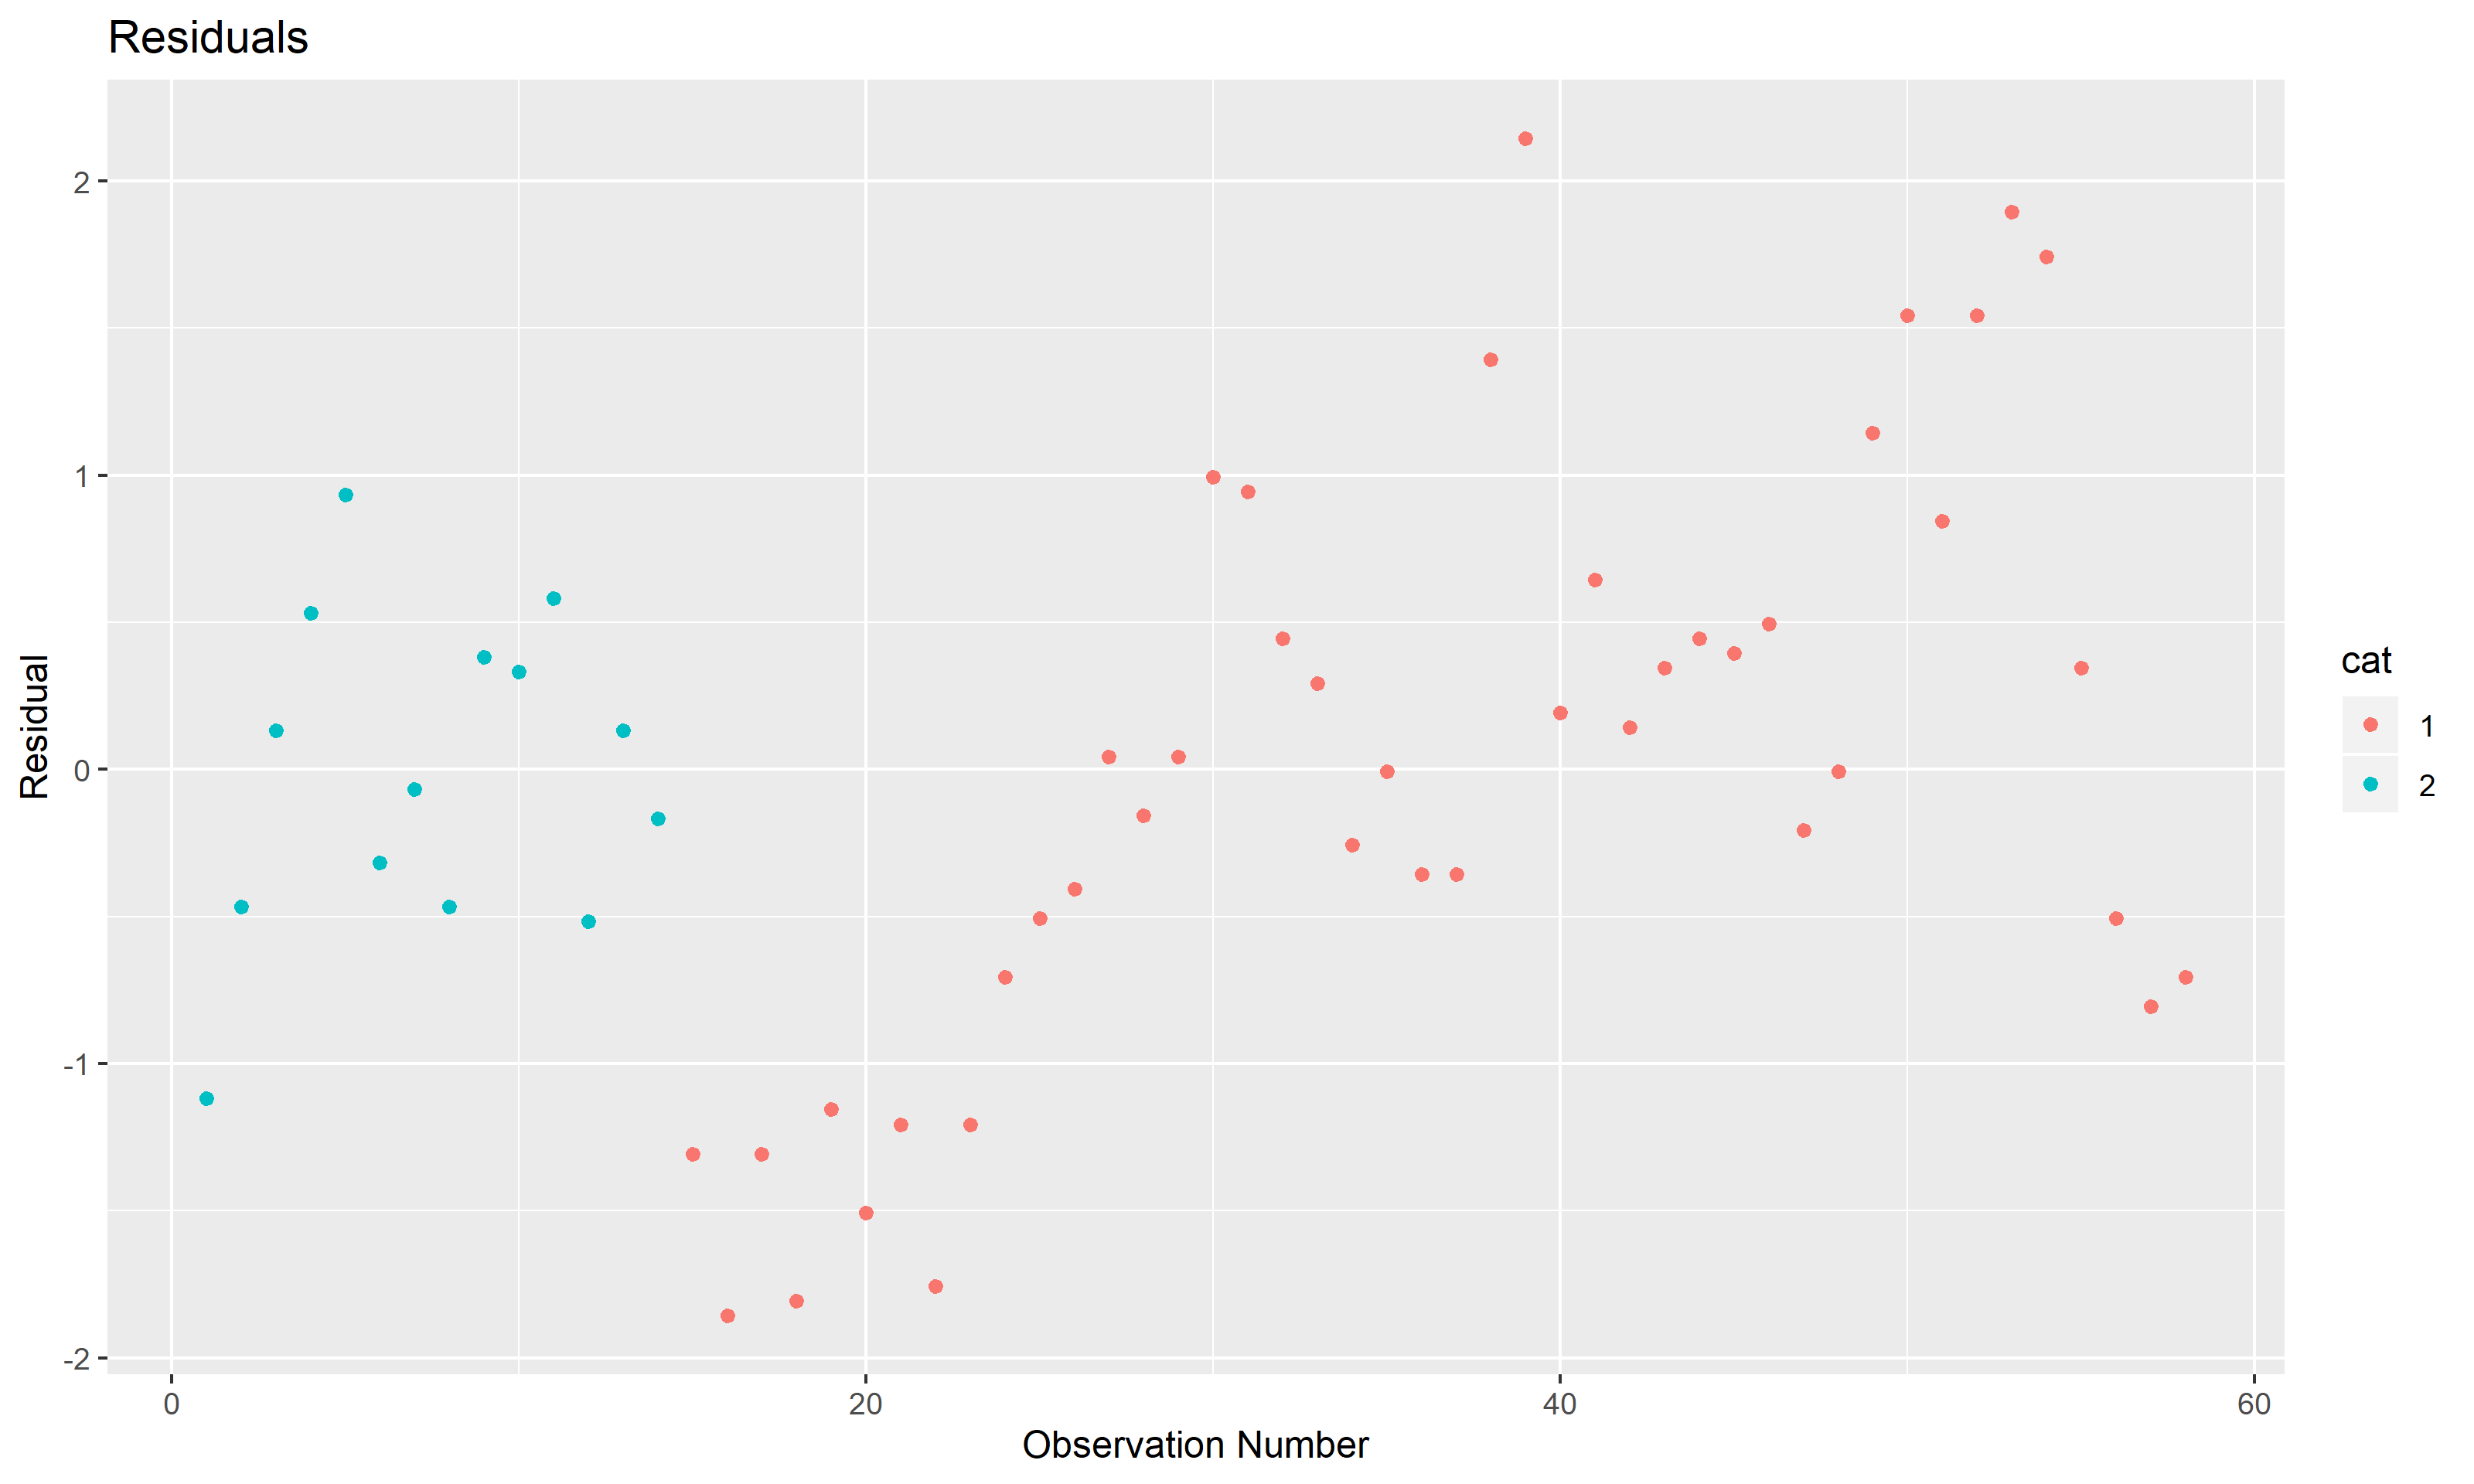
\includegraphics[width=\linewidth]{../plots/06_mod1_resid_1.png}
	\caption{Plot of residuals, we can see that the two groups show a pattern where the first month has higher variance than the second.}
	\label{fig:7}
\end{figure}

\begin{figure}[h!]
	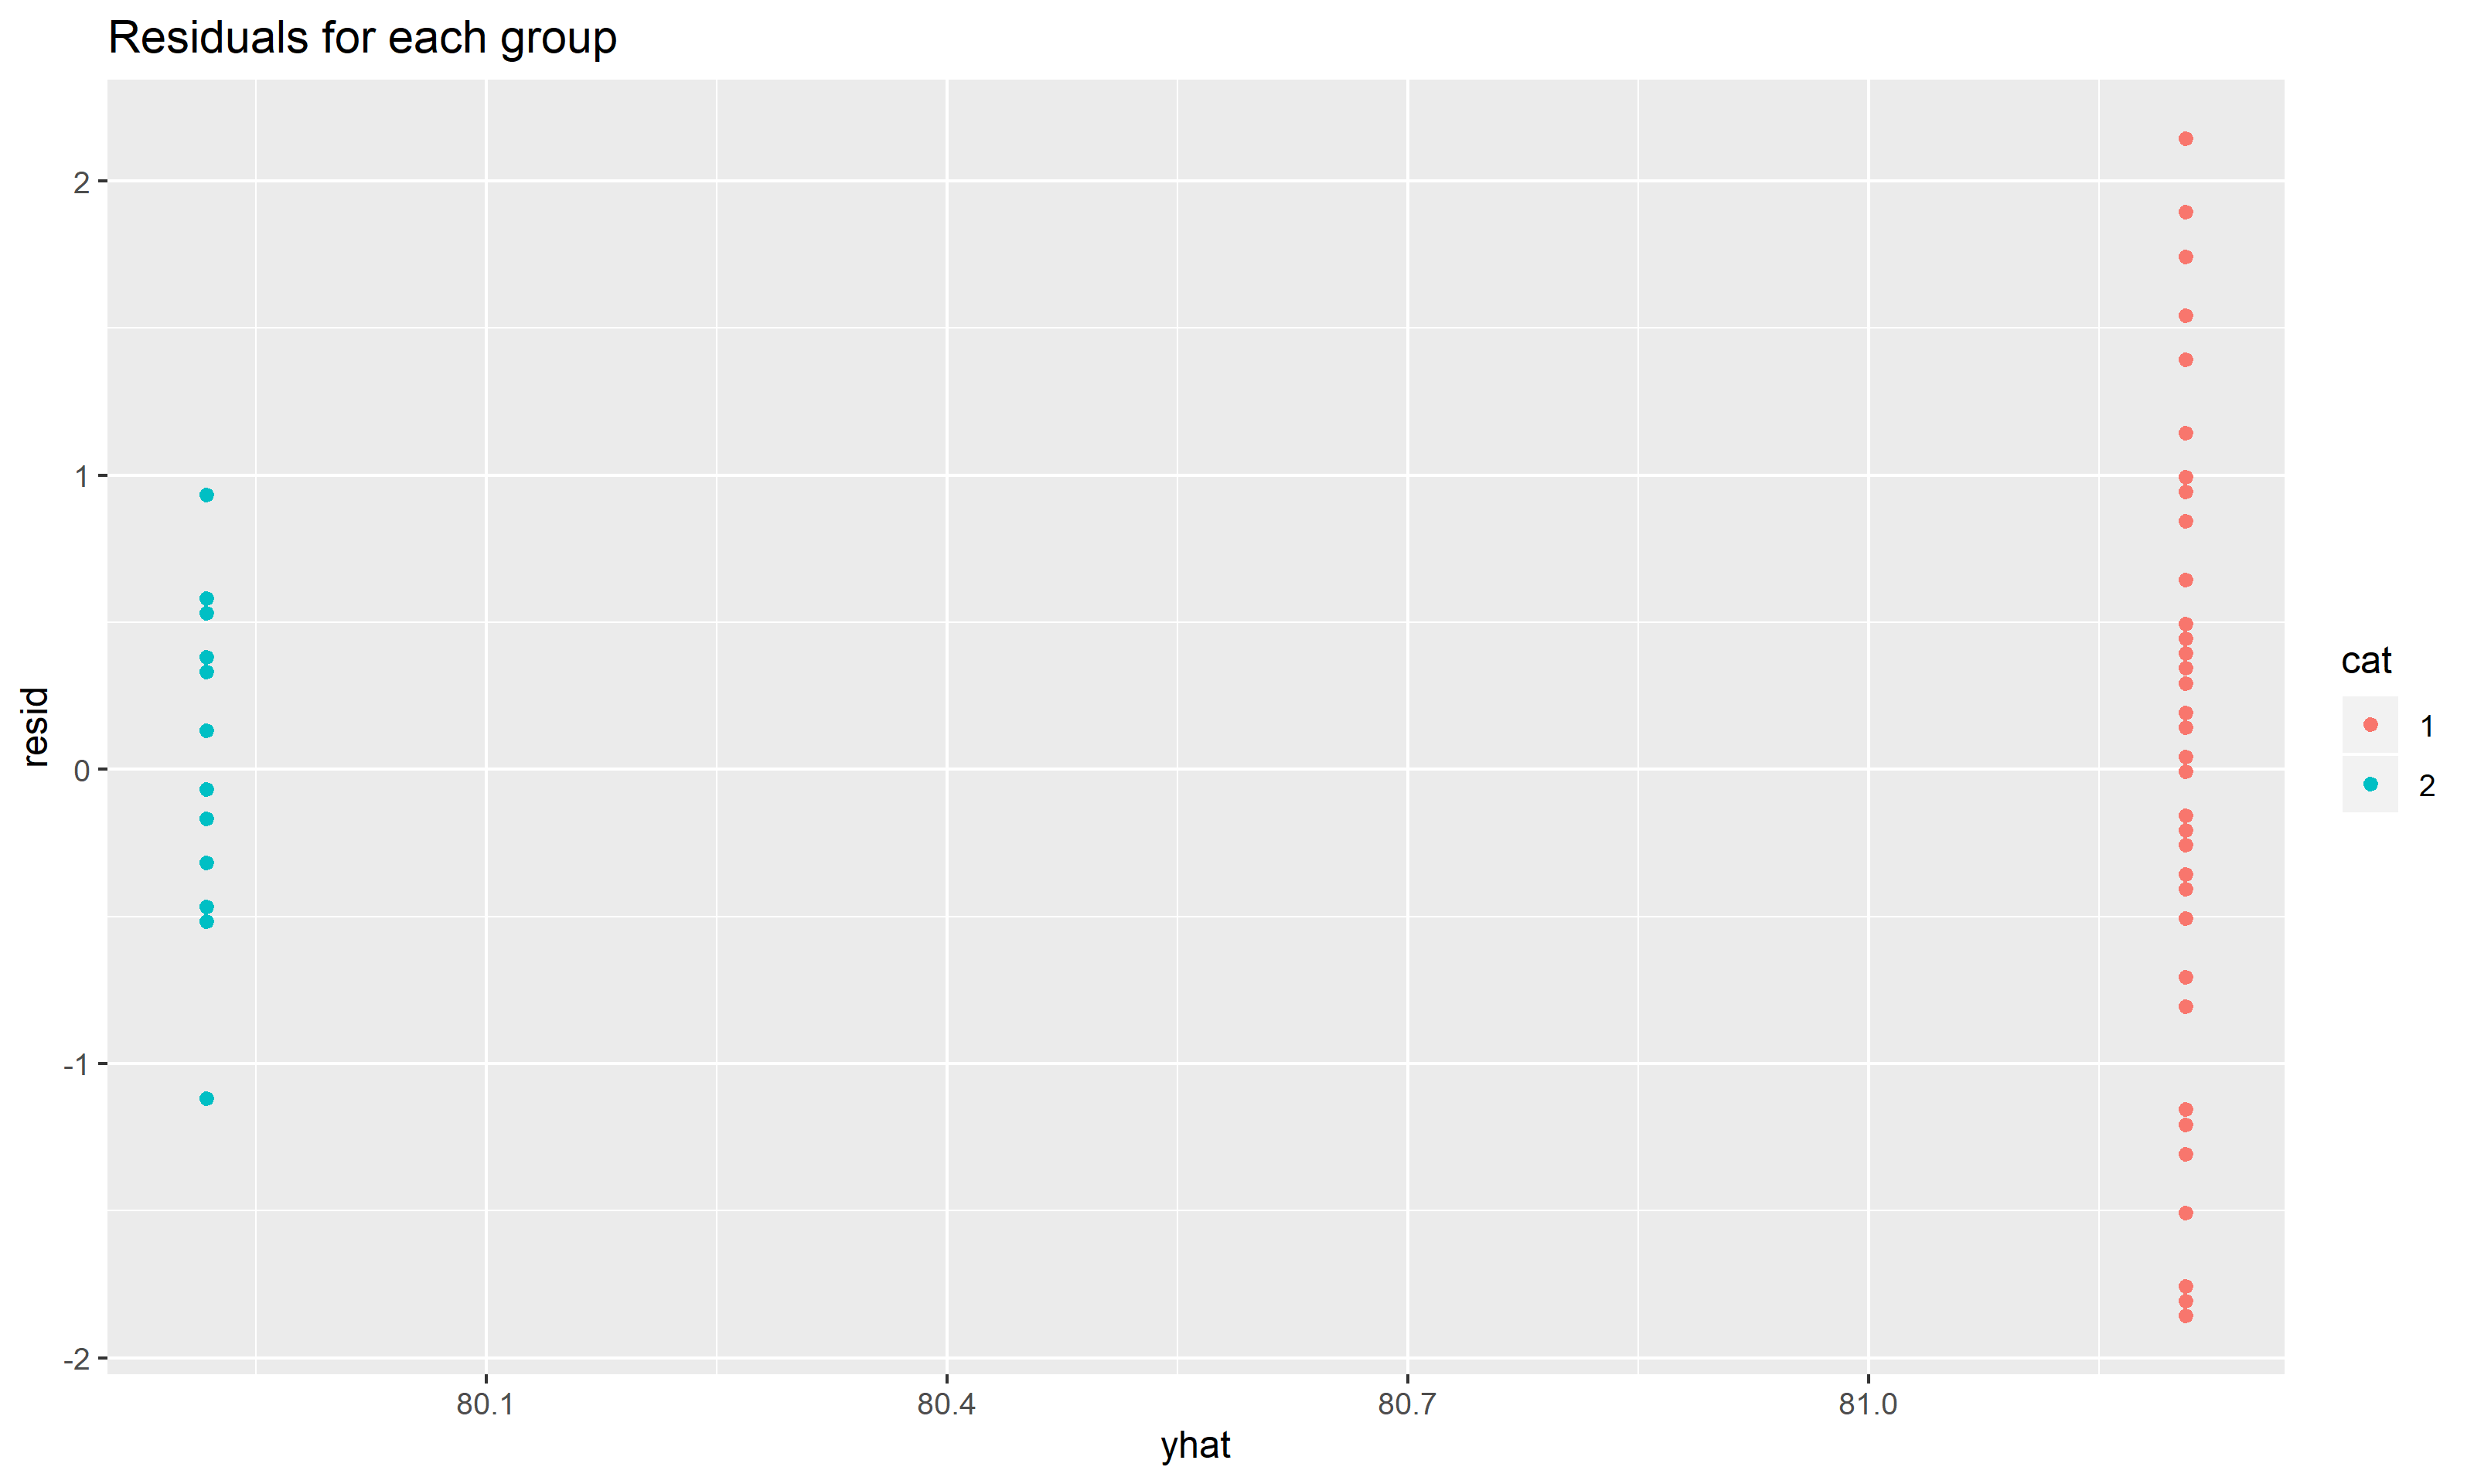
\includegraphics[width=\linewidth]{../plots/06_mod1_resid_2.png}
	\caption{Plot of residuals, we can see that the two groups show a pattern where the first month has higher variance than the second.}
	\label{fig:8}
\end{figure}

\begin{figure}[h!]
	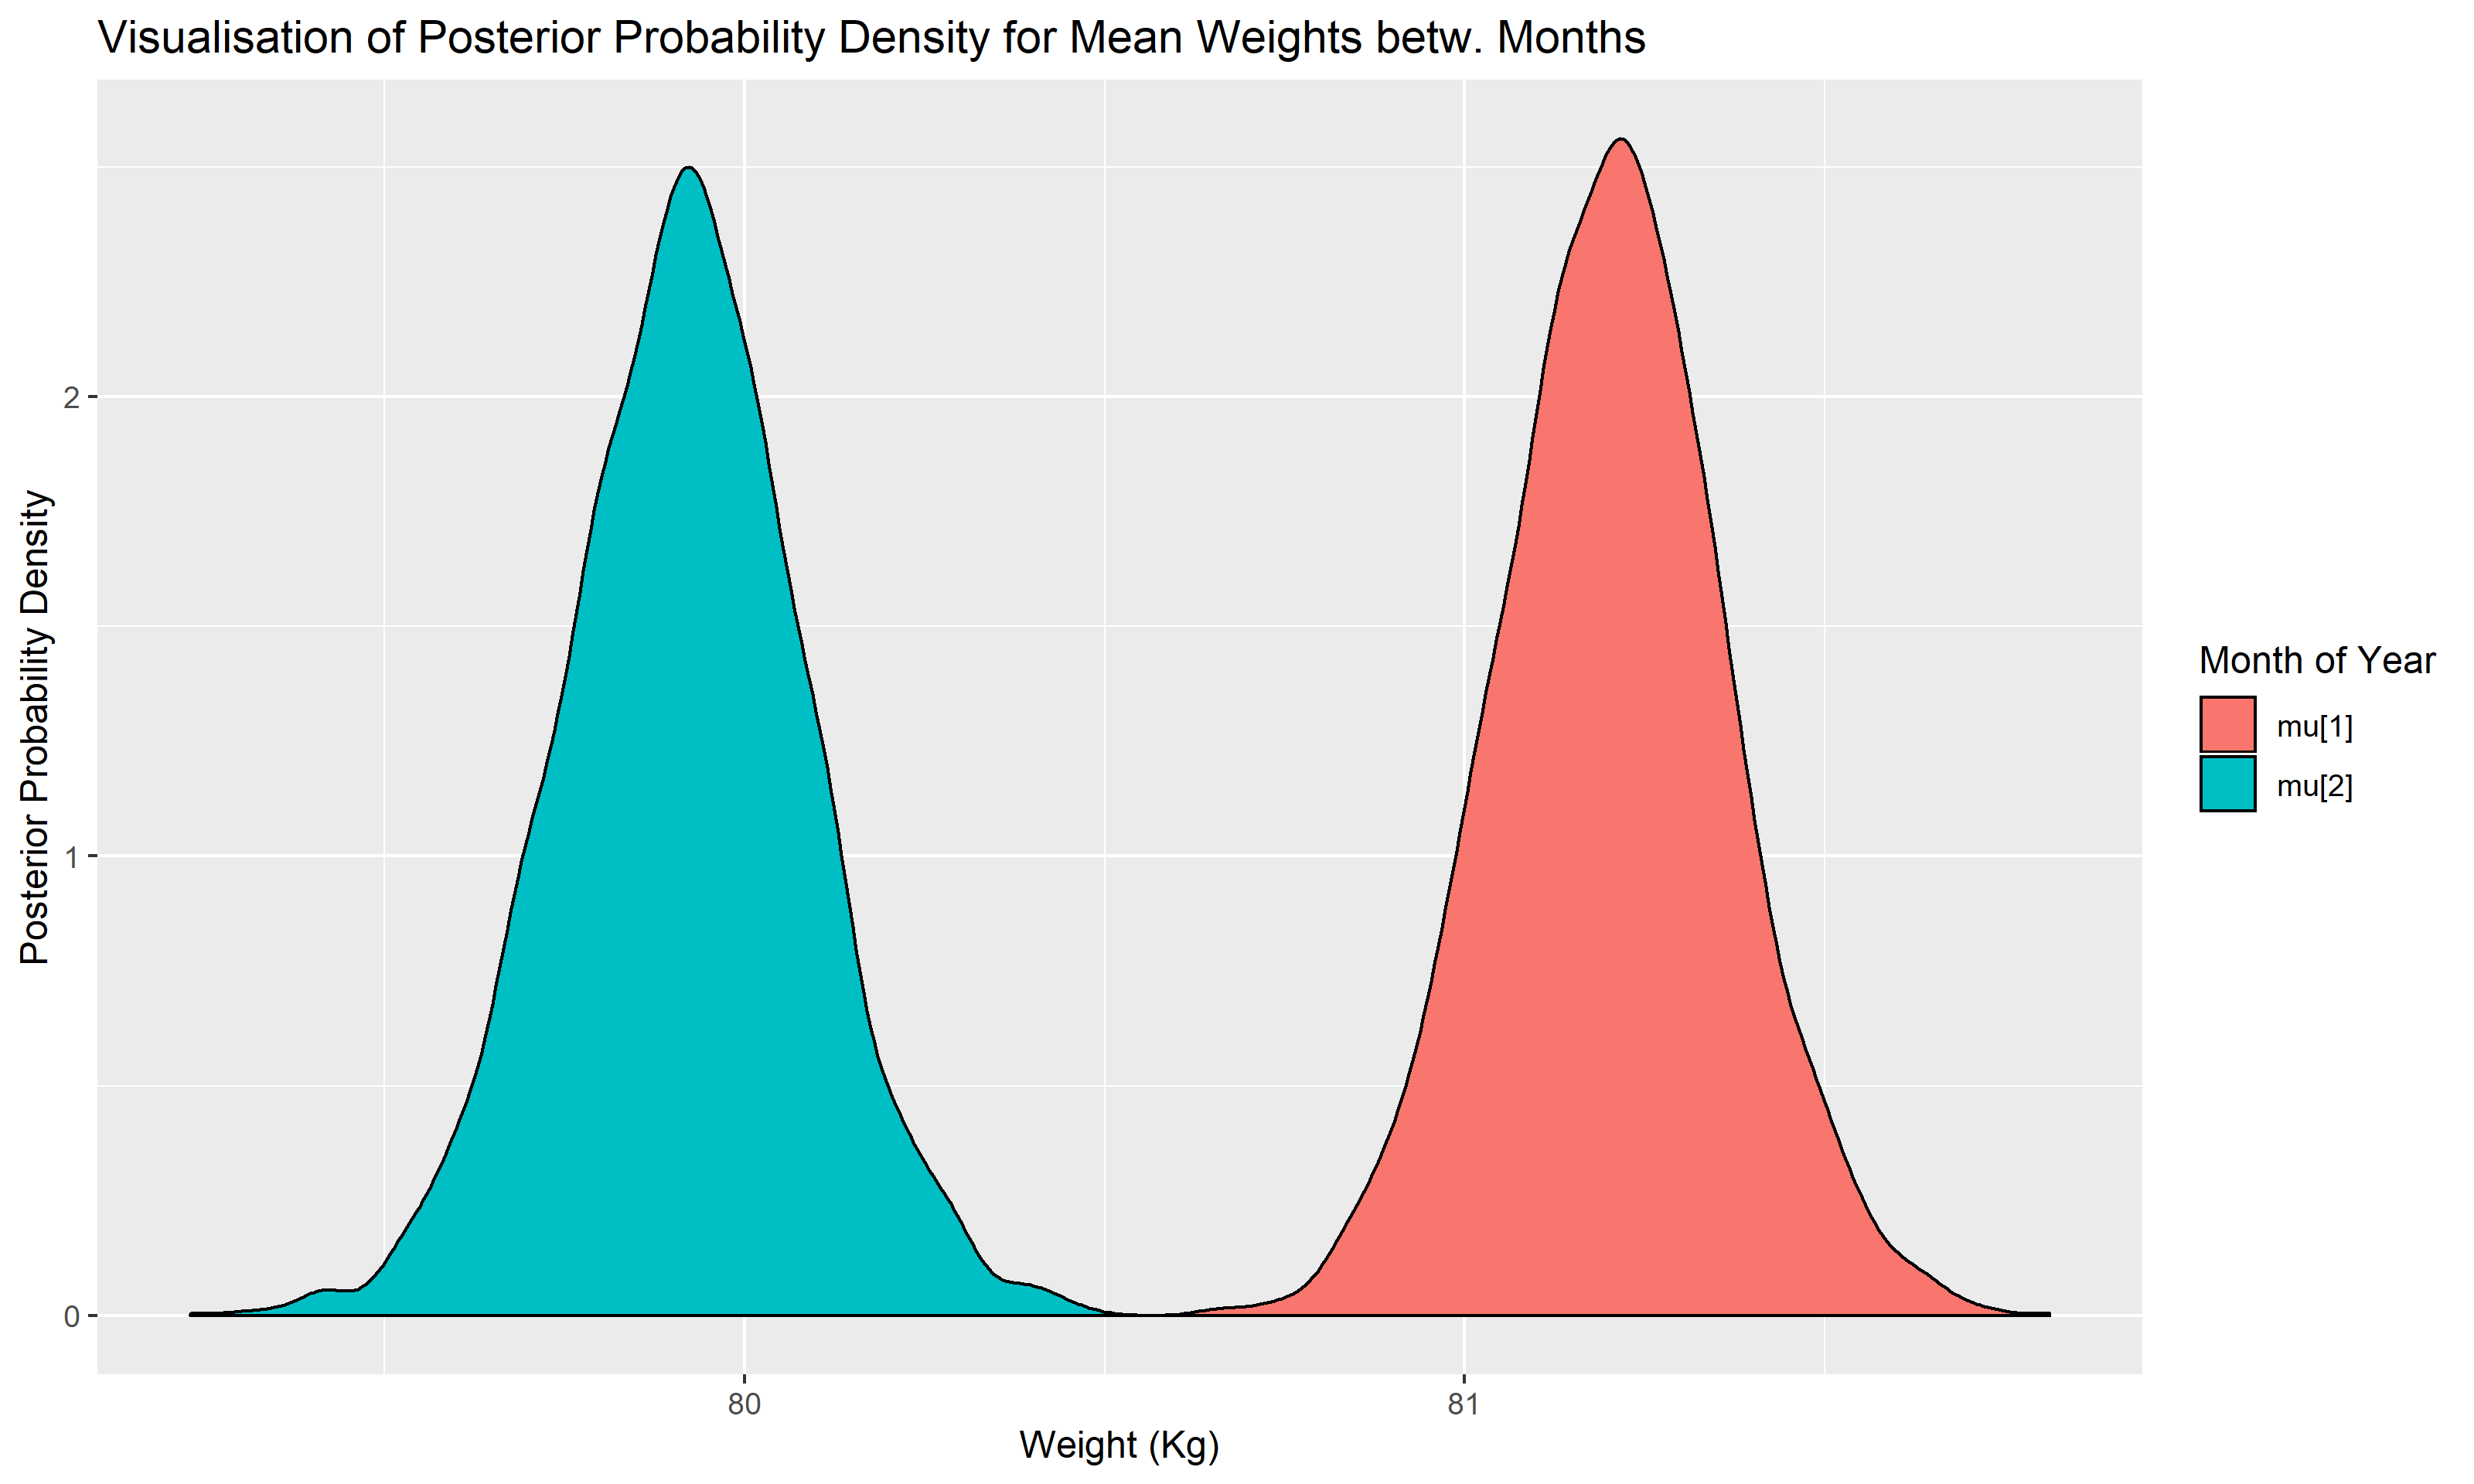
\includegraphics[width=\linewidth]{../plots/07_post_dist_weights.png}
	\caption{Density plots for the posterior samples for the first and second means. We can see very little overlap between the two distributions which strongly
	suggests that the weights between the two months are meaningful.}
	\label{fig:9}
\end{figure}

\end{document}